\documentclass[]{revdetua}
\usepackage{graphicx} % Required for inserting images

\Header{Volume}{5}{Dezembro}{2023}{0}

\title{Advanced Algorithms - Second Project \linebreak Maximum Clique Problem}
\author{Gonçalo Machado Nmec 98359}
\date{December 2023}

\begin{document}

\maketitle

\begin{abstract}
This report presents an algorithmic solution for the Maximum Clique Problem, alongside its formal analysis regarding its efficiency, a discussion of the obtained results, a comparison with the algorithms developed in the first project and predictions for large problem instances. This problem is addressed by the course "Advanced Algorithms" at the University of Aveiro. The proposed algorithm is a Monte Carlo algorithm. The chosen coding language was Python.
\end{abstract}

\begin{resumo}% Note: in Portuguese
Este relatório apresenta uma solução algorítmica para o problema Clique Máximo, assim como a análise formal da sua eficiência, uma discussão dos resultados obtidos, uma comparação com os algoritmos desenvolvidos no primeiro projeto e previsões para problemas de maior escala. Este problema é abordado pelo curso "Algoritmos Avançados" na Universidade de Aveiro.O algoritmo proposto é classificado como Monte Carlo.A linguagem de programação escolhida foi Python.
\end{resumo}

\begin{keywords}
Graph, Clique, Maximum Clique, Edges, Vertices, Monte Carlo Algorithm, Las Vegas Algorithm, Randomized Algorithm
\end{keywords}

\begin{palavraschave}
Grafo, Clique, Clique Máximo, Arestas, Vértices, Algoritmo Monte Carlo, Algoritmo Las Vegas, Algoritmo Randomizado
\end{palavraschave}

\section{Introduction}
This report is part of the second project of "Advanced Algorithms". The goal of the project was to design and test a randomized algorithm to solve the \textbf{Maximum Clique} problem.

The following sections describe the problem and some key concepts, explain how the graphs were created, how the algorithm works and analyse the performance and computation complexity of the algorithm. For the analysis, both a formal computational analysis and an experimental computational analysis were done, with the latter consisting of a series of experiments, for successively larger problem instances, where the \textbf{number of basic operations}, the \textbf{execution time} and the \textbf{number of solutions / attempts tested} were registered. The analysis were compared with each other and an attempt to estimate the execution time of the algorithms for much larger problem instances was made. The results of the algorithm developed for this project were also compared with the results from the algorithms developed in the previous project, in order to see the accuracy between algorithms and the trade-off between the accuracy of an algorithm and its running time. 

Alongside the report there were also the files containing the code developed, the graphs used in the experiments ,the results derived from the algorithms developed in the first and second project as well as the comparisons between them. In order to run the code, we first generate the graphs, then run the file with the chosen algorithm. The commands used to run the code are the following: \linebreak

\$ python generate\_graphs.py 

\$ python randomized\_algorithm.py

\$ python greedy\_heuristics.py

\section{Maximum Clique Problem}

As said before, the goal of the project was to solved the \textbf{Maximum Clique Problem}, which asks us to find a maximum clique for a given undirected graph G(V, E), with n vertices and m edges. A clique of G is a subset of vertices, all adjacent to each other, i.e., defining a complete subgraph of G. A maximum clique is a clique with the largest possible number of vertices. Example: in a social network, a clique is a subset of people who all know each other.

An important fact is that a graph can have more than one maximum clique, which happens if there are two cliques with the same size and there are no cliques with bigger size than them. In this case, the algorithms will return one of the maximum cliques.

The problem given to us also described the characteristics of the graph instances that would be used by the algorithms, which are the following:

\begin{itemize}
\item Graph vertices are 2D points on the XoY plane, with integer-valued coordinates between 1 and 100.
\item Graph vertices should neither be coincident nor too close.
\item The number of edges sharing a vertex is randomly determined.
\item Use 12.5\%, 25\%, 50\%, and 75\% of the maximum number of edges for the number of vertices.
\item Graph edges are unweighted and undirected.
\item The graphs need to be generated using a student number as the seed.
\end{itemize}

To construct a graph, and following the rules given to us, we first need to generate the list of vertices. Each vertex has a randomly generated tuple of integer-valued coordinates between 1 and 100 and an ID associated to them. One of the rules states that the vertices should neither be coincident nor too close, and while the first part is certain ( two vertices are either coincident or not), the second part is subjective to interpretation. As such, we considered that two vertices were "too close" if the distance between them was less than 7. Before being added to the list, each vertex was compared to every other vertex to check if the distance was below the minimum defined. For this problem we decided that the number of vertices of a graph would be between 4 and 150, since more than this would not be feasible for the algorithms to use.

After generating the list of vertices, we need to generated the list of edges. One of the rules states that a percentage of the maximum number of edges needs to be used when generating the list, so for each number of vertices in a graph, we created 4 graphs, each using a different percentage of the maximum number of edges. The maximum number of edges is calculated with the formula: \( n(n-1)/2 \) where n is the number of vertices in the graph. Each edge is generated by randomly picking two vertices and seeing if an edge between the two exists, and if not, add a tuple with the ids of the two vertices to the list of edges.

After generating each graph, and in order to store them for later use, we create a JSON with two fields:

\begin{itemize}
    \item vertices - Contains a JSON object where each pair has the id of the vertex as the key and the coordinates as the value
    \item edges - Contains a list of edges, with each edge being a list of the ids of the two vertices that the edge is connected to.
\end{itemize}

The object is then saved with a name that follows the format {number of vertices}\_vertices\_{percentage of maximum edges}\_edge\_percentage. An example of the object would be:
\linebreak \linebreak
 \{"vertices": {"0": [20, 70], "1": [72, 75], "2": [48, 23], "3": [48, 52], "4": [74, 43]}, "edges": [[1, 0], [4, 1], [4, 2], [1, 2], [4, 0]]\}
\linebreak

To load the graph we simply read the content of the JSON and using \textit{Networkx} create a networkx.Graph object and insert each vertex and each edge into the object.

After using an algorithm to get the maximum cut of the graph, we obtain a maximum clique of the graph, which consists in a list of the ids that are in the maximum clique. For example, the maximum clique of the graph used in the previous example is [0,1,4].

\section{Analysis of Algorithm Efficiency}

To analyse the efficiency of an algorithm, we will do so as a function of the algorithm's input size. In our case, it is the size of list of vertices in the generated graphs.

As per requested in the problem given to us, we will use the \textbf{number of basic operations}, the \textbf{execution time} and the \textbf{number of solutions / attempts tested} to measure the algorithm's efficiency. From these three values, it is worth mentioning that the execution time is not the best parameter to use in order to assess the efficiency, since it largely depends on the machine were the algorithm is ran, the language the algorithm was written on and the use or not of parallelization.

The \textbf{number of basic operations} is the best parameter to analyse the efficiency, since it does not depend on external factors, it only depends on the algorithm itself. A basic operation is the operation contributing the most to the total running time of an algorithm usually being the most time consuming operation in the algorithm's innermost loop. The basic operation of the algorithm will be described in the section explaining the algorithm.

To note that for the kind of algorithm developed in this project, a randomized algorithm, the use of the accuracy of the algorithm is also an excellent way to evaluate the potential use of the algorithm, since the algorithm as a max number of basic operations it can do. 

When analysing the efficiency of an algorithm, we should also understand that the algorithm might have different number of basic operations for graphs of the same input size. Due to this, we will consider:

\begin{itemize}
    \item Worst-case scenario - The worst-case efficiency of an algorithm is its efficiency for the worst-case input of size n (for which the algorithm runs the longest among all possible inputs of that size)
    \item Best-case scenario - The best-case efficiency of an algorithm is its efficiency for the best-case input of size n (for which the algorithm runs the fastest among all possible inputs of that size)
\end{itemize}

Each of the cases will be addressed with more detail in the section pertaining the algorithm.

\section{Randomized Algorithm}

Randomized algorithms are computational methods that intentionally incorporate randomness in their processes to solve problems. Unlike traditional deterministic algorithms, which produce consistent outputs for a given input, randomized algorithms introduce an element of chance during execution. This intentional use of randomness allows these algorithms to provide approximate solutions, often with associated probabilities of correctness. They are particularly useful in situations where exact solutions may be challenging or computationally expensive. By leveraging randomness strategically, randomized algorithms offer a flexible and efficient approach to problem-solving, finding applications across various domains, from optimization to graph algorithms.

Randomized algorithms are mostly divided in two categories: Las Vegas and Monte Carlo. Las Vegas algorithms always produce correct results, but their runtime can vary. They use randomness to improve efficiency, and while the output is guaranteed to be accurate, the time taken might differ between runs. On the other hand, Monte Carlo algorithms may produce incorrect results with a certain probability but have a fixed and usually faster runtime. Despite the potential for errors, Monte Carlo algorithms are valuable when approximate solutions are acceptable, and their efficiency makes them suitable for various computational tasks, such as statistical simulations and optimization problems. The algorithm developed belongs to the Monte Carlo category.

Before using the algorithm, we first load all graphs that will be used, which for the purpose of comparing results with the algorithms of the previous project, included graphs from 4 to 33 vertices. We then go through all graphs and call the algorithm for each graph.

The algorithm employs a combination of random sampling and local search. The algorithm iteratively samples subsets of vertices, performs a local search within each subset, and dynamically adjusts the size of the sampled vertices based on the results. To prevent revisiting the same solutions, it maintains a set of tested solutions. The main loop continues until a maximum number of operations is reached or a maximum-sized clique covering all nodes in the graph is found. The local search function explores cliques by greedily adding nodes that maintain the clique property. The algorithm returns the best-found clique, which might or might not be a maximum clique, the total number of operations performed, and the number of attempts made to discover a maximum clique.

Some important details about the algorithm that were developed in order to follow the specifications of the project:
\begin{itemize}
    \item \textbf{Ensuring that no such solutions are tested more than once.} - As mentioned previously, this was done by maintaining a set with all tested solutions, meaning that if the same vertex sample was done, it would simply generate a new one.
    \item \textbf{Deciding when to stop testing candidate solutions of a certain size and start testing larger or smaller solutions.} - This was done by increasing or decreasing the size of the vertex sample in relation to the size of the clique found. If the size of the discovered clique is more than half of the current sample size, it increases the sample size of the next sample. If the size of the discovered clique is less than half of the current sample size, it decreases the sample size of the next sample, but never to a smaller size than the best-known clique, since the maximum clique of the graph can only be bigger or the same size as the best-known clique
    \item \textbf{Deciding when to stop testing altogether} - This happened in 3 possible cases :
        \begin{itemize}
            \item The algorithm reached the maximum number of basic operations defined
            \item The algorithm found a clique with the same number of vertices as the graph, which is the biggest clique possible in a graph
            \item The algorithm tested all possible combinations of vertices, which are \( 2^n \) with n being the number of vertices in the graph
        \end{itemize}
\end{itemize}

The basic operation of this algorithm is the act of choosing a vertex from the vertices of the graph. The selected vertex is then added if it is not already in the sample, and if it is already in the sample the algorithm will simply continue. This task is considered a basic operation since the selection of random vertices might select the same vertex multiple times or even create the same samples multiple times, making the algorithm spend a lot of time in the creation of the samples than on the other parts of the algorithm.

the best-case scenario is when the graph itself is a clique. In this case, the algorithm would make 2 loops: one where it generates a sample with half of the graph vertices, and another were it generates a sample with all of the graph vertices. In the best-case scenario, the creation of the samples would also be the best-case scenario, which would be the algorithm choosing the vertices of both samples without a single repetition, which would mean that the complexity of the best case scenario would be O\( n/2 + n \), which simplifies to O\(3n/2\) with n being the number of vertices in the graph.    

The worst-case scenario is the same as the average-case scenario, which is when the algorithm reaches the maximum number of operations permitted. In this case the returned clique might not be the maximum clique of the graph. The complexity of this would be O\(m\), with m being the maximum number of operations defined.

As we can understand from the previous assessments, the algorithm in most cases reaches the maximum number of operations, meaning that it has an expected end time that only depends on the maximum number of operations permitted, but the result given might not be correct. We can also expect the algorithm, with the same maximum number of operations permitted, to give less accurate results the bigger the problem instance, since it will have bigger samples, which lead to more operations done per sample. The algorithm is also expected to have more accuracy the bigger the maximum number of operations is, for the same graphs, since it is able to test more possible solutions. The number of attempts tested might vary for the same graph or for graphs with the same number of vertices since the sampling of the vertices uses randomness, which can lead to more operations done to create a sample with the same size.

\section{Results}

\subsection{Experiments}

For the experiments of the algorithm, graphs with vertices between 4 and 33 vertices and 12.5\%, 25\%, 50\%, and 75\% of the maximum number of edges for the number of vertices were used. The number 33 as the most vertices a graph could have was chosen so it would be possible to compare the results of this algorithm to the exhaustive search algorithm developed in the first project. It is worth nothing that due to the nature of the algorithm developed in this project, much larger graphs could be used, but an assertion of the validity of the result would not be possible.

As for the maximum number of operations, the values tested were 1000, 2500, 5000, 10000, 20000, 100000, 500000, 1000000, 2500000 and 5000000. To note that the most time the algorithm ran was less than 6 seconds.

The following table presents the algorithm, the maximum number of operations, the number of correct results and its accuracy.

\begin{table}[!ht]
    \centering
    Algorithms Accuracy
    \begin{tabular}{|l|l|l|l|}
    \hline
        Algorithm & Max. Op. & Correct Res. & Acc. (\%) \\ \hline
        Exhaustive & --- & 119 & 1.0 \\ \hline
        Greedy & --- & 45 & 37.82 \\ \hline
        Randomized & 1000 &74 & 62.18 \\ \hline
        Randomized & 2500& 77 & 64.71 \\ \hline
        Randomized & 5000 & 88 & 73.95 \\ \hline
        Randomized & 10000 & 90 & 75.63 \\ \hline
        Randomized & 20000 & 93 & 78.15 \\ \hline
        Randomized & 100000 & 104 & 87.39 \\ \hline
        Randomized & 500000 & 105 & 88.24 \\ \hline
        Randomized & 1000000 & 108 & 90.76 \\ \hline
        Randomized & 2500000 & 110 & 92.44 \\ \hline
        Randomized & 5000000 & 108 & 90.76 \\ \hline
    \end{tabular}
\end{table}

By analysing the table, when can clearly see a relation between the number of max operations and the accuracy of the algorithm, where the larger the maximum operations allowed, the greater the accuracy. This matches the empirical analysis made previously.

It is also possible to see that the algorithm performed better with a maximum of operations of 2500000 than with 5000000. This is simply due to the randomness of the algorithm and should not be considered as basis for any proof. In another experiment with the same parameters, the results might not and probably will not be the same, but the previously mentioned relation between the number of maximum operations and the accuracy of the algorithm will stay true.

It is worth noting that even with only 1000 maximum operations, the randomized algorithm has a greater accuracy than the greedy algorithm from the previous project.

\subsection{Basic Operations}

In terms of basic operations, since the only two cases where the algorithm stops before reaching the maximum number of operations is if the graph itself is a clique, which is extremely unlikely, or if all combinations have been tested, which is also very unlikely, the number of operations of the algorithm is equal to or a little bigger than the maximum number of operations. The fact that it can be a little bit bigger derives from the algorithm only checking if the maximum number of operations is reached at the beginning of every loop, and not after every basic operation.

When comparing the number of operations of the randomized algorithm with different maximum number of operations, Fig 2, with the number of operations of the exhaustive algorithm, Fig 1, we can see a clear difference between the rapid growth of the exhaustive algorithm operations and the constant value of the randomized algorithm operations, which was expected. 

\begin{figure}[h]
    \centering
    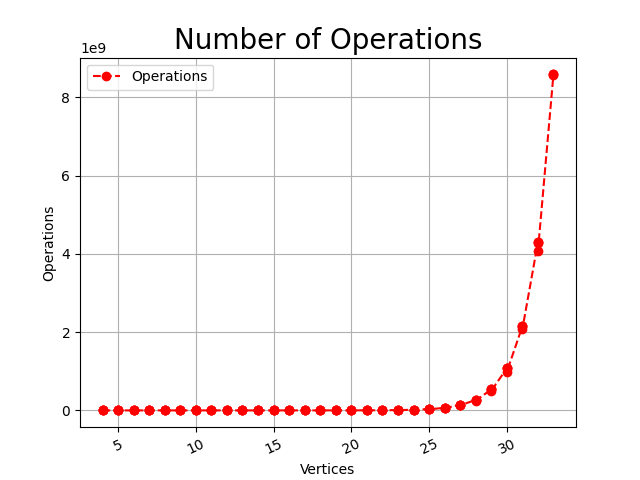
\includegraphics[width=8cm]{operations_exhaustive.png}
    \caption{Exhaustive Search Operations}
\end{figure}

\begin{figure}[h]
    \centering
    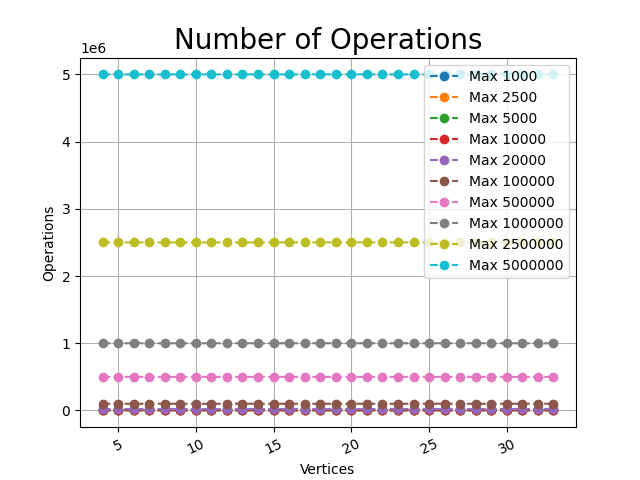
\includegraphics[width=8cm]{operations_randomized.png}
    \caption{Randomized Algorithm Operations}
\end{figure}

\subsection{Attempts Tested}

\begin{figure}[h]
    \centering
    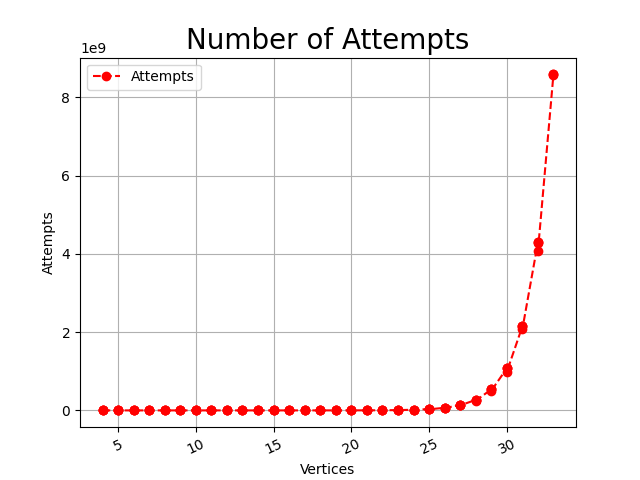
\includegraphics[width=8cm]{attempts_exhaustive.png}
    \caption{Exhaustive Search Attempts}
\end{figure}

\begin{figure}[h]
    \centering
    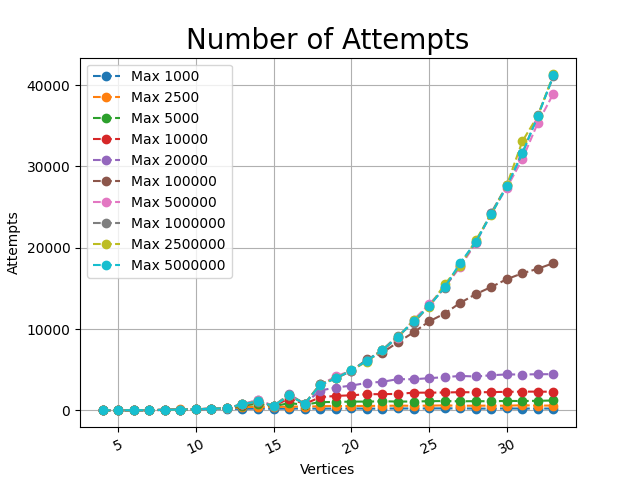
\includegraphics[width=8cm]{attempts_randomized.png}
    \caption{Randomized Algorithm Attempts}
\end{figure}

By analysing Fig 3, which has the number of attempts tested by the exhaustive algorithm, with Fig 4, which has the number of attempts tested by the randomized algorithm with the different maximum number of operations, we can see, as we concluded in the formal analysis, that the number of attempts tested by the randomized algorithm is lower than by the exhaustive algorithm, with the difference increasing the more vertices the graph has.

We can also see that the number of attempts of the randomized algorithm is larger the bigger the maximum number of operations, which matches the formal analysis.

\subsection{Execution Time}

\begin{figure}[h]
    \centering
    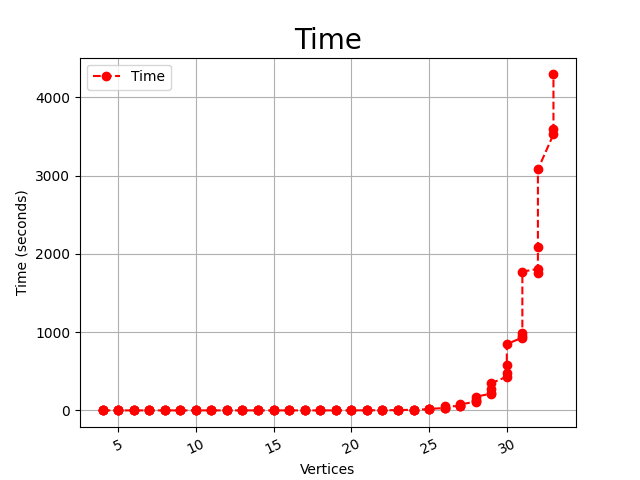
\includegraphics[width=8cm]{time_exhaustive.png}
    \caption{Exhaustive Search Execution Time}
\end{figure}

\begin{figure}[h]
    \centering
    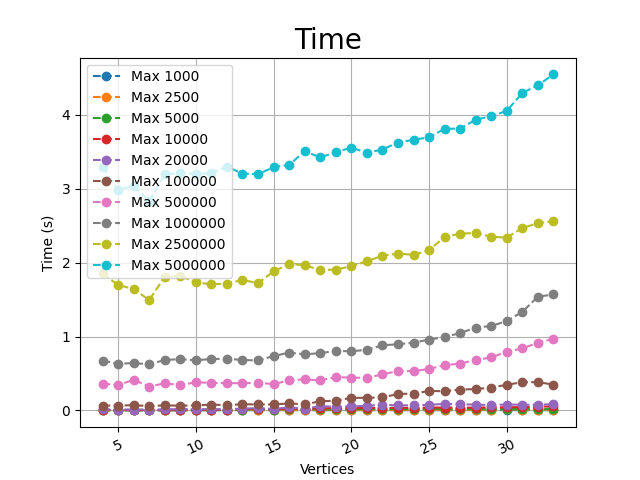
\includegraphics[width=8cm]{time_randomized.png}
    \caption{Randomized Algorithm Execution Time}
\end{figure}

By analysing Fig 5, which has the execution time of the exhaustive algorithm, with Fig 6, which has the execution time of the randomized algorithm with the different maximum number of operations, we can see that they are magnitudes different from each other, with the difference between them increasing the more vertices the graph has.

We can also notice a very small difference in execution times between the different maximum operations of the randomized algorithm. This is simply due to the algorithm executing more operations.

It is also possible to notice some variation in the execution time of the algorithm with the same maximum number of operations, where this variation is mostly in the positive side, meaning that the execution time slightly increases the more vertices the graph has. This is due to the size of the samples that are created being larger the more vertices the graph has.

\section{Conclusion}

In conclusion, we can now see the advantages and disadvantages of randomized algorithms over deterministic algorithms. While randomized algorithms offer a quick and efficient way of getting results within a known time frame, the result might not be the correct one. On the other hand, the exhaustive algorithm always reaches an optimal solution, but it is very expensive in terms of complexity, due to its exponential growth.

Finally, randomized algorithms, due to their random nature, should be evaluated with the probability of returning a correct result, with parameter tuning being done to achieve the biggest possibility possible without compromising execution time.

\begin{thebibliography}{00}

\bibitem{b1} Wikipedia (2023). \textit{Maximal clique} [Online]. Available: \url{https://en.wikipedia.org/wiki/Clique_problem#:~:text=%5Bedit%5D-,Finding%20a%20single%20maximal%20clique,-%5Bedit%5D}
\bibitem{b2} Wolfram Alpha \textit{Maximal clique Problem} [Online]. Available: \url{https://mathworld.wolfram.com/MaximalClique.html}
\bibitem{b3} Wikipedia (2023) \textit{Randomized Algorithm} [Online]. Available: \url{https://en.wikipedia.org/wiki/Randomized_algorithm}
\bibitem{b4} Wikipedia (2023) \textit{Monte Carlo Algorithm} [Online]. Available: \url{https://en.wikipedia.org/wiki/Monte_Carlo_algorithm}
\end{thebibliography}

\end{document}